\section{Qualitätssicherung}

\begin{defi}{Qualitätsmanagement}
    Unter \emph{Qualitätsmanagement} (QM) versteht man \emph{alle Tätigkeiten der Gesamtführungsaufgabe}, welche die \emph{Qualitätspolitik}, \emph{Ziele} und \emph{Verantwortungen festlegen}, sowie diese durch Mittel wie Qualitätsplanung, Qualitätslenkung, Qualitätssicherung und Qualitätsverbesserung im Rahmen des Qualitätsmanagements verwirklichen.
\end{defi}

\begin{defi}{Qualitätssicherung}
    Unter \emph{Qualitätssicherung} (QS) versteht man \emph{alle geplanten und systematischen Tätigkeiten}, die innerhalb des Qualitätsmanagementsystems verwirklicht sind, und die wie erforderlich dargelegt werden, um \emph{angemessenes Vertrauen} zu schaffen, dass eine Einheit die \emph{Qualitätsanforderungen erfüllen} wird.

    Jedes Dokument, das im Verlaufe der Softwareerstellung bzw. Softwarewartung erzeugt bzw. verändert wird, sollte einer Qualitätssicherung unterliegen.
    Dazu zählen alle Produkte und Zwischenergebnisse der jeweiligen Phase (Anforderungsdefinition, Entwurfsspezifikation, Programmcode, Dokumentation, etc.).
\end{defi}

\begin{defi}{Prinzipien der Qualitätssicherung}
    \begin{tabularx}{\textwidth}{|>{\bfseries}l|>{- }X|}
        \hline
        Prinzip                & \multicolumn{1}{l}{\bfseries Erläuterung}                                                                                                                                                                \\
        \hline
        \hline
        Zielgerichtet          & muss durch projektspezifische Ziele getrieben werden                                                                                                                                                     \\
                               & Festlegung von Anforderungen für Q-Merkmale                                                                                                                                                              \\
        \hline
        Quantitativ            & erfordert Anwendung quantitativer Methoden zur Bewertung der Qualität von Produkten und Prozessen                                                                                                        \\
                               & Festlegung und Messung von Kennzahlen für objektive Beurteilung                                                                                                                                          \\
        \hline
        Maximal konstruktiv    & so viele Fehler wie möglich durch geeignete Sprachen, Methoden, Werkzeuge im Vorfeld verhindern                                                                                                          \\
                               & Statt mangelhafte Qualität durch analytische Qualitätssicherung a posteriori aufzudecken, werden konstruktive Maßnahmen ergriffen, um die Entwicklung hochqualitativer Software a priori sicherzustellen \\
        \hline
        Frühzeitig             & QS muss in den frühen Phasen (so früh wie möglich) eingesetzt werden, um Fehler so früh wie möglich zu erkennen und zu beheben                                                                           \\
        \hline
        Integriert             & QS nahtlos in den Softwareprozess integrieren und in allen Phasen einsetzen                                                                                                                              \\
                               & Nicht erst fertige Dokumente prüfen                                                                                                                                                                      \\
        \hline
        Unabhängig bzw. Extern & Analytische QS nicht nur unter Kontrolle der Entwickler durchführen                                                                                                                                      \\
                               & QS muss (auch) von einer unabhängigen Organisationseinheit durchgeführt werden                                                                                                                           \\
        \hline
        Werkzeugunterstützt    & Prüfung soweit möglich automatisieren                                                                                                                                                                    \\
        \hline
        Skaliert               & Kosten und Nutzen von QS-Maßnahmen beobachten                                                                                                                                                            \\
        \hline
    \end{tabularx}
\end{defi}

\begin{defi}{Klassifizierung von QS-Verfahren}
    Qualitätssicherungsmaßnahmen in der Softwareentwicklung beziehen sich auf:
    \begin{itemize}
        \item Das \emph{Produkt} Software (produktorientiert)
        \item Den \emph{Prozess} der Softwareentwicklung (prozessorientiert)
    \end{itemize}

    Man teilt daher Qualitätssicherungsmaßnahmen (QSM) auf in
    \begin{itemize}
        \item \emph{Konstruktive Ansätze}
              \begin{itemize}
                  \item Aktivitäten mit positiver Auswirkung auf Qualität
                  \item \emph{Während} der Erstellung von Software-Produkten
                  \item Fehlervermeidungsstrategie
                  \item \enquote{Vorbeugen besser als Heilen}
              \end{itemize}
        \item \emph{Analytische Ansätze}
              \begin{itemize}
                  \item Testen, Verifikation, Messen (über Qualitätsmerkmale)
                  \item \emph{Nach} Erstellung von Software-Produkten
                  \item Fehlerfindungsstrategie
              \end{itemize}
    \end{itemize}
\end{defi}

\begin{bonus}{Konstruktive QS-Verfahren}
    \begin{itemize}
        \item \textbf{Richtlinien}
              \begin{itemize}
                  \item Prozessrichtlinien
                  \item Standards für Dokumente, Coding-Guidelines
                  \item Gliederungsschema für Lasten- und Pflichtenheft
              \end{itemize}
        \item \textbf{Methoden}
              \begin{itemize}
                  \item Vorgehensmodelle (SCRUM, etc.)
                  \item Abarbeitung von Checklisten
                  \item Schulungen
              \end{itemize}
        \item \textbf{Werkzeuge}
              \begin{itemize}
                  \item Für Projektmanagement
                  \item Case-Tools
              \end{itemize}
        \item \textbf{Sprachen}
              \begin{itemize}
                  \item UML
              \end{itemize}
        \item \textbf{Entwurfsmuster} für Softwarearchitektur
        \item etc.
    \end{itemize}
\end{bonus}

\begin{defi}{Review}
    Unter einem \emph{Review} versteht man einen manuell durchgeführten statischen Prüfprozess.
    Ein Review wird häufig gleichgesetzt mit dem \enquote{Gegenlesen des eigenen Codes von Kollegen}.

    Man unterscheidet generell zwischen:
    \begin{itemize}
        \item Code-Reviews (Fokus: Quelltext)
        \item Architektur-Reviews (Fokus: Design- und technische Dokumente)
    \end{itemize}

    Das Hauptziel besteht darin, Probleme an einem Arbeitsergebnis oder Dokument zu erkennen, die nicht werkzeuggestützt erkannt werden können:
    \begin{itemize}
        \item semantische bzw. logische Fehler
        \item fehlende Einhaltung von Standards
        \item Abweiwchung von Referenzdokumenten
    \end{itemize}

    Nebenbei erzielen Reviews aber auch:
    \begin{itemize}
        \item Verbreitung der Wissensbasis im Team
        \item Lernen von Arbeitsmethoden der KollegInnen
        \item Konsenzbildung (Team-Verantwortung)
    \end{itemize}
\end{defi}

\subsection{Tests}

\begin{defi}{Klassifikation von Tests}
    \begin{itemize}
        \item \textbf{Abstraktion}
              \begin{itemize}
                  \item Black-Box-Test (funktional)
                  \item White-Box-Test (strukturell)
              \end{itemize}
        \item \textbf{Granularität}
              \begin{itemize}
                  \item Testen im Kleinen (Testen einzelner Komponenten)
                  \item Testem im Großen (Testen von Teilsystemen oder des gesamten Systems)
              \end{itemize}
        \item \textbf{Zeit}
              \begin{itemize}
                  \item Komponententest (Unit-Test) (nach der Implementierung einer Komponente)
                  \item Integrationstest (nach einem Komponententest)
                  \item Systemtest (vom Auftragnehmenden vor dem Abnahmetest)
                  \item Abnahmetest (von Auftraggebendem bei der Auslieferung)
              \end{itemize}
    \end{itemize}
\end{defi}

\subsubsection{Black-Box-Tests}

\begin{defi}{Black-Box-Test}
    \emph{Black-Box-Test} bezeichnet eine Methode des Softwaretests.
    Hierbei werden Tests anhand der Spezifikation bzw. Anforderung entwickelt.
    Dies bedeutet, dass Tests ohne Kenntnisse über die innere Funktionsweise bzw. Implementierung des zu testenden Systems entwickelt werden.

    Das zu testende Programm wird also als Black Box behandelt.
    Nur nach außen sichtbares Verhalten fließt in den Test ein.
\end{defi}

\begin{defi}{Äquivalenzklassenbildung}
    Ziel der Bildung von \emph{Äquivalenzklassen} ist es, eine hohe Fehlerentdeckungsrate mit einer möglichst geringen Anzahl von Testfällen zu erreichen. Die Äquivalenzklassen sind also bezüglich Ein- und Ausgabedaten ähnliche Klassen bzw. Objekte, bei denen erwartet wird, dass sie sich gleichartig verhalten.

    Das Wesen der Äquivalenzklassenbildung besteht darin, die gesamten Eingabedaten und Ausgabedaten eines Programms in Gruppen von Äquivalenzklassen zu unterteilen, so dass man annehmen kann, dass mit jedem beliebigen Objekt einer Klasse die gleichen Fehler wie mit jedem anderen Objekt dieser (Äquivalenz-)Klasse gefunden werden.

    Vorgehen:
    \begin{enumerate}
        \item Mögliche Eingaben in Bereiche aufteilen, sogenannte \emph{Klassen}
              \begin{itemize}
                  \item Alle Elemente einer klasse zeigen identisches Verhalten
              \end{itemize}
        \item Zulässige und unzulässige Klassen trennen
        \item Für jede Klasse mindestens einen \emph{Repräsentanten} wählen für die Testdaten
        \item Vereinigung der Äquivalenzklassen sollte der gesamte Wertebereich sein.
    \end{enumerate}
\end{defi}

\begin{example}{Äquivalenzklassenbildung}
    Gegeben sei folgende Funktion:
    \begin{lstlisting}
        /**
        Setzt fuer ein uebergebenes Pokemon einen Spitznamen.
        *
        * @param pokemon Das Pokemon, dessen Spitzname gesetzt werden soll.
        * @param name Der Spitzname des Pokemon, dabei gilt:
        * - der Name anderer Pokemon-Arten ist verboten
        * - der Name muss mindestens 3 und maximal 20 Zeichen lang sein
        * - der Name darf nur aus Buchstaben bestehen
        * @return true, wenn der Spitzname gesetzt werden konnte, false sonst.
        * @throws IllegalArgumentException wenn name kein String ist.
        * @throws IllegalArgumentException wenn pokemon kein Pokemon ist.
        */
        boolean setSpitzname(Pokemon pokemon, String name) {
    \end{lstlisting}

    Wir erhalten folgende Äquivalenzklassen:\footnote{Wir gehen davon aus, dass \texttt{pikachu} ein korrekt erstelles Objekt vom Typ \texttt{Pokemon} ist.}

    \begin{tabularx}{\textwidth}{|l|l|l|X|X|}
        \hline
        \multirow{2}{*}{\bfseries \#} & \multirow{2}{*}{\bfseries Äquivalenzklasse} & \multirow{2}{*}{\bfseries Typ}   & \multicolumn{2}{c|} {\bfseries Repräsentant}                            \\ \cline{4-5}
                                      &                                             &                                  & \texttt{pokemon}                             & \texttt{name}            \\
        \hline
        0                             & Normalfall                                  & (Zulässig, \texttt{true})        & \texttt{pikachu}                             & \texttt{"Bobo"}          \\
        1                             & Spitzname verboten                          & (Unzulässig, \texttt{false})     & egal                                         & \texttt{"Glumanda"}      \\
        2                             & Spitzname zu kurz                           & (Unzulässig, \texttt{false})     & egal                                         & \texttt{"P"}             \\
        3                             & Spitzname zu lang                           & (Unzulässig, \texttt{false})     & egal                                         & \texttt{"Pikaa...aachu"} \\
        4                             & Spitzname ungültig                          & (Unzulässig, \texttt{false})     & egal                                         & \texttt{"P1k4chUwU"}     \\
        5                             & Spitzname \texttt{null}                     & (Unzulässig, \texttt{Exception}) & egal                                         & \texttt{null}            \\
        6                             & Pokemon \texttt{null}                       & (Unzulässig, \texttt{Exception}) & \texttt{null}                                & egal                     \\
        \hline
    \end{tabularx}
\end{example}

\begin{defi}{Grenzwertanalyse}
    Die \emph{Grenzwertanalyse} ist ein Spezialfall der Äquivalenzklassenanalyse.

    Sie ist aus der Beobachtung entstanden, dass Fehler besonders häufig an den \enquote{Rändern} der Äquivalenzklassen auftreten.
    Daher werden hier nicht beliebige Werte getestet, sondern sogenannte Randwerte oder Grenzwerte.

    Weiterhin können auch leere bzw. fehlende Eingaben, Randelemente, Extremwerte und \enquote{ungünstige} Eingaben geprüft werden.
\end{defi}

\begin{example}{Grenzwertanalyse}
    \begin{tabularx}{\textwidth}{|l|l|l|X|}
        \hline
        \multirow{2}{*}{\bfseries \#} & \multirow{2}{*}{\bfseries Typ} & \multicolumn{2}{c|} {\bfseries Repräsentant}                                                                   \\ \cline{3-4}
                                      &                                & \texttt{pokemon}                             & \texttt{name}                                                   \\
        \hline
        2                             & Unzulässig                     & pikachu                                      & \texttt{``''}                                                   \\
        2                             & Unzulässig                     & pikachu                                      & \texttt{"P"}                                                    \\
        2                             & Unzulässig                     & pikachu                                      & \texttt{"Pi"}                                                   \\
        2                             & Unzulässig                     & pikachu                                      & \texttt{"Pik"}                                                  \\
        0                             & Zulässig                       & pikachu                                      & \texttt{"Pika"}                                                 \\
        0                             & Zulässig                       & pikachu                                      & \texttt{"Pikaaaaaaaaaaaaaachu"}                                 \\
        3                             & Unzulässig                     & pikachu                                      & \texttt{"Pikaaaaaaaaaaaaaaachu"}                                \\
        3                             & Unzulässig                     & pikachu                                      & \texttt{"Pika...achu"} (Länge: \texttt{Integer.MAX\_VALUE - 1}) \\
        3                             & Unzulässig                     & pikachu                                      & \texttt{"Pika...aachu"} (Länge: \texttt{Integer.MAX\_VALUE})    \\
        \hline
    \end{tabularx}
\end{example}

\subsubsection{White-Box-Tests}

\begin{defi}{White-Box-Test}
    Der Begriff \emph{White-Box-Test} bezeichnet eine Methode des Software-Tests, bei der die Tests mit Kenntnissen über die innere Funktionsweise des zu testenden Systems entwickelt werden.

    Im Gegensatz zum Black-Box-Test ist für diesen Test also ein Blick in den Quellcode gestattet.
    D.h., es wird am Code geprüft.
\end{defi}

\begin{defi}{Kontrollflussorientiertes Testverfahren}
    Ein Beispiel für einen White-Box-Test ist ablaufbezogenes Testen (\emph{kontrollflussorientierte Testverfahren}), bei welchem der Ablaufgraph im Vordergrund steht.

    Qualitätskriterium des Tests ist es, sicherzustellen, dass Testfälle in Bezug auf die Überdeckung des Quellcodes gewisse Hinlänglichkeitskriterien erfüllen.
    Gängig sind dabei u. a. folgende Maße (bzw. Qualitätskriterien):
    \begin{itemize}
        \item Zeilenüberdeckung: Ausführung aller Quellcode-Zeilen
        \item Anweisungsüberdeckung bzw. Knotenüberdeckung: Ausführung aller Anweisungen
        \item Zweigüberdeckung bzw. Kantenüberdeckung: Durchlaufen aller möglichen Kanten von Verzweigungen des Kontrollflusses
        \item Bedingungsüberdeckung bzw. Termüberdeckung (mehrere Varianten): Durchlaufen aller möglichen ausschlaggebenden Belegungen bei logischen Ausdrücken in Bedingungen
        \item Pfadüberdeckung (mehrere Varianten): Betrachtung der Pfade durch ein Modul
    \end{itemize}
\end{defi}

\begin{defi}{Anweisungsüberdeckungstest}
    \emph{Anweisungsüberdeckungstests} bzw. Statement Coverage testen jede Anweisung mindestens ein Mal.

    Wurde jede Anweisung in einem Programm mindestens einmal ausgeführt, spricht man von \emph{vollständiger Anweisungsüberdeckung}.

    Wurde vollständige Anweisungsüberdeckung erreicht, dann steht fest, dass kein toter Code (Anweisungen, die niemals durchlaufen werden) im Programm existiert.

    Der \emph{Anweisungsüberdeckungsgrad} $C_0$ bestimmt sich wie folgt:
    \[
        C_0 = \frac{\text{Anzahl der durchlaufenen Anweisungen}}{\text{Gesamtzahl der Anweisungen}}
    \]
\end{defi}

\begin{example}{Anweisungsüberdeckungstest}
    Gegeben sei der folgende Kontrollflussgraph:
    \begin{center}
        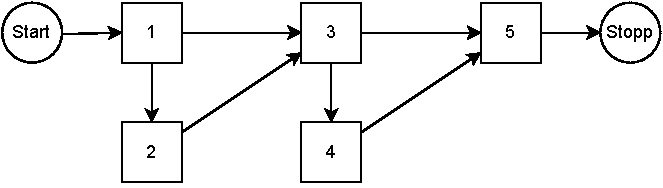
\includegraphics[width=0.5\textwidth]{includes/figures/example_kontrollfluss_base.pdf}
    \end{center}

    Für diesen Kontrollflussgraphen kann die Anweisungsüberdeckung mit einem Testfall erreicht werden:
    \begin{itemize}
        \item \texttt{Start, 1, 2, 3, 4, 5, Stopp}
    \end{itemize}

    Wir erhalten:
    \begin{center}
        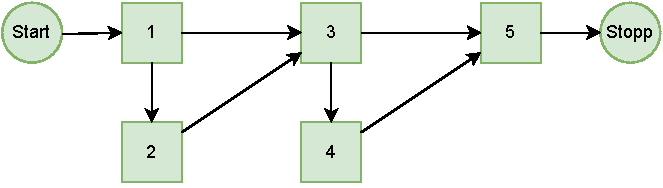
\includegraphics[width=0.5\textwidth]{includes/figures/example_kontrollfluss_anweisung.pdf}
    \end{center}
\end{example}

\begin{defi}{Zweigüberdeckungstest}
    Der \emph{Zweigüberdeckungstest} bzw. Branch Coverage umfasst den Anweisungsüberdeckungstest vollständig.

    Für den Zweigüberdeckungstest  müssen strengere Kriterien erfüllt werden als beim Anweisungsüberdeckungstest.
    Im Bereich des kontrollflussorientierten Testens wird der Zweigüberdeckungstest als Minimalkriterium angewendet.

    Mit Hilfe des Zweigüberdeckungstests lassen sich nicht ausführbare Programmzweige aufspüren.
    Anhand dessen kann man dann Softwareteile, die oft durchlaufen werden, gezielt optimieren.

    Weitaus komplizierter erweist sich das Zweigüberdeckungsmaß.
    In dem Fall, dass alle Knoten gleich bewertet sind, verzichtet man auf die Betrachtung der Abhängigkeiten untereinander.
    Dadurch entsteht kein linearer Zusammenhang zwischen der erreichten Überdeckungsrate und dem Verhältnis zwischen der Anzahl der dazu benötigten Testfälle und der eigentlichen Anzahl der Testfälle, die für die 100-prozentige Zweigüberdeckung notwendig sind.

    Um den Zweigüberdeckungstest zu verbessern, wird ein Zweig, der abhängig von einem anderen Zweig ist, nicht weiter berücksichtigt.
    Die Zweige, die nicht abhängig sind, werden als primitiv bezeichnet.

    Daher ergibt sich für das Überdeckungsmaß:
    \[
        C_{\text{primitiv}} = \frac{\text{Anzahl der ausgeführten primitiven Zweige}}{\text{Anzahl der primitiven Zweige}}
    \]
\end{defi}

\begin{example}{Zweigüberdeckungstest}
    Gegeben sei der folgende Kontrollflussgraph:
    \begin{center}
        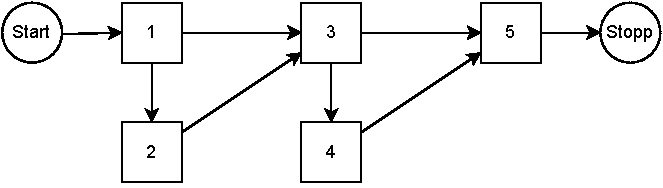
\includegraphics[width=0.5\textwidth]{includes/figures/example_kontrollfluss_base.pdf}
    \end{center}

    Eine Zweigüberdeckung ist dann gegeben mit:
    \begin{itemize}
        \item \texttt{Start, 1, 2, 3, 4, 5, Stopp}

              \vspace{1em}
              \begin{center}
                  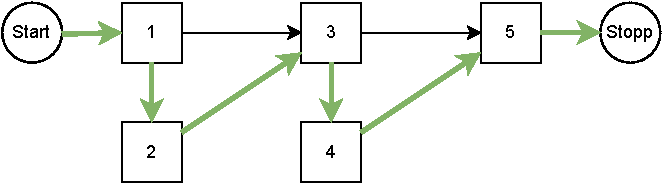
\includegraphics[width=0.5\textwidth]{includes/figures/example_kontrollfluss_zweig_1.pdf}
              \end{center}
        \item \texttt{Start, 1, 3, 5, Stopp}

              \vspace{1em}
              \begin{center}
                  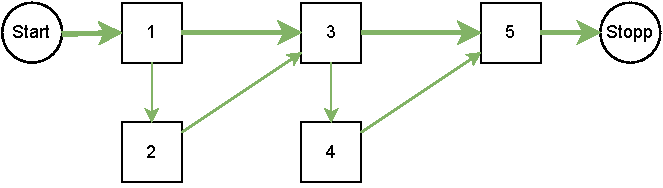
\includegraphics[width=0.5\textwidth]{includes/figures/example_kontrollfluss_zweig_2.pdf}
              \end{center}
    \end{itemize}
\end{example}

\begin{defi}{Pfadüberdeckungstest}
    Beim \emph{Pfadüberdeckungstest} bzw. Path Covrage werden im Kontrollflussgraphen die möglichen Pfade vom Startknoten bis zum Endknoten betrachtet.

    \begin{itemize}
        \item \textbf{vollständiger Pfadüberdeckungstest}:
              \begin{itemize}
                  \item Es werden alle möglichen Pfade getestet.
                  \item Problem: Bei Programmen mit Schleifen kann es extrem viele Pfade geben.
              \end{itemize}
        \item \textbf{Boundary-Interior-Pfadüberdeckungstest}:
              \begin{itemize}
                  \item Im Prinzip wie der vollständige Pfadüberdeckungstest, nur dass nun die Schleifendurchläufe auf höchstens zwei reduziert werden.
                  \item Für jede Schleife gibt es zwei Gruppen von Pfaden:
                        \begin{itemize}
                            \item Boundary-Test: Jede Schleife wird keinmal und genau einmal betreten und alle Pfade im Schleifenkörper werden einmal abgearbeitet.
                            \item Interior-Test: Das Schleifeninnere gilt als getestet, wenn alle Pfade, die bei zweimaligem Durchlaufen möglich sind, abgearbeitet wurden.
                        \end{itemize}
              \end{itemize}
        \item \textbf{strukturierter Pfadüberdeckungstest}:
              \begin{itemize}
                  \item Im Prinzip wie der Boundary-Interior-Pfadüberdeckungstest, nur dass nun die Anzahl der Schleifendurchläufe auf eine vorgegebene Zahl $n$ reduziert wird.
              \end{itemize}
    \end{itemize}
\end{defi}

\begin{example}{Pfadüberdeckungstest}
    Gegeben sei der folgende Kontrollflussgraph:
    \begin{center}
        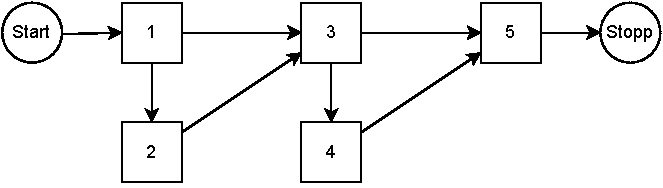
\includegraphics[width=0.5\textwidth]{includes/figures/example_kontrollfluss_base.pdf}
    \end{center}

    Eine Pfadüberdeckung ist dann gegeben mit:
    \begin{itemize}
        \item \texttt{Start, 1, 2, 3, 4, 5, Stopp}

              \vspace{1em}
              \begin{center}
                  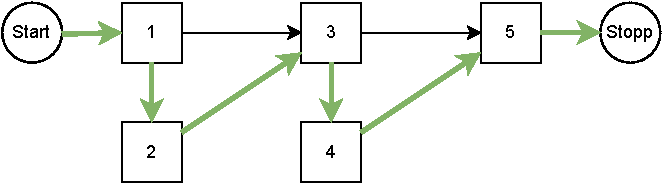
\includegraphics[width=0.5\textwidth]{includes/figures/example_kontrollfluss_pfad_1.pdf}
              \end{center}
        \item \texttt{Start, 1, 3, 5, Stopp}

              \vspace{1em}
              \begin{center}
                  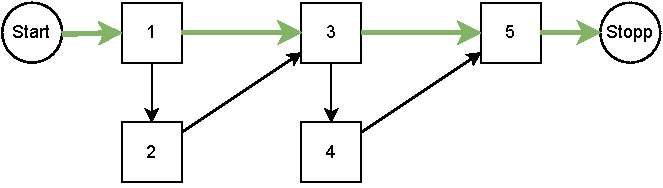
\includegraphics[width=0.5\textwidth]{includes/figures/example_kontrollfluss_pfad_2.pdf}
              \end{center}
        \item \texttt{Start, 1, 3, 4, 5, Stopp}

              \vspace{1em}
              \begin{center}
                  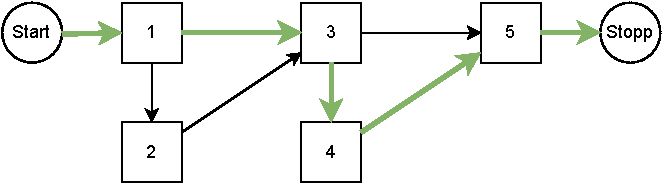
\includegraphics[width=0.5\textwidth]{includes/figures/example_kontrollfluss_pfad_3.pdf}
              \end{center}
        \item \texttt{Start, 1, 2, 3, 5, Stopp}

              \vspace{1em}
              \begin{center}
                  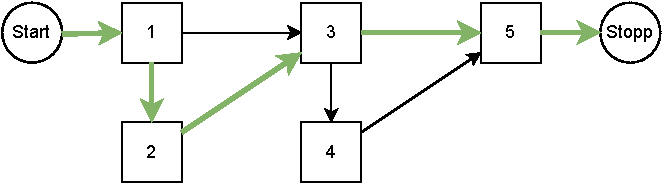
\includegraphics[width=0.5\textwidth]{includes/figures/example_kontrollfluss_pfad_4.pdf}
              \end{center}
    \end{itemize}
\end{example}

\begin{defi}{Bedingungsüberdeckungstest}
    Das Problem der bisherigen Überdeckungstests ist, dass zusammengesetzte, hierarchische Bedingungen nicht ausreichend getestet werden.

    \begin{itemize}
        \item \textbf{Einfachbedingungsüberdeckungstest}:
              \begin{itemize}
                  \item Jede atomare Bedingung einer Entscheidung muss einmal mit \texttt{true} und einmal mit \texttt{false} getestet werden.
              \end{itemize}
        \item \textbf{Mehrfachbedingungsüberdeckungstest}:
              \begin{itemize}
                  \item Dieser Test betrachtet alle atomaren Bedingungen einer Bedingung.
                  \item Wenn $n$ atomare Bedingungen in der Bedingung stehen, dann werden $2^{n}$ Kombinationen gebildet.
              \end{itemize}
        \item \textbf{minimaler Mehrfachbedingungsüberdeckungstest}:
              \begin{itemize}
                  \item Diese Version erstellt mehr Testfälle als der Einfachbedingungsüberdeckungstest und weniger als der Mehrfachbedingungsüberdeckungstest, indem jede Bedingung (atomar und zusammengestellt) zu \texttt{true} und zu \texttt{false} evaluiert wird.
                  \item Die logische Struktur wird hierbei berücksichtigt und der Zweigüberdeckungstest ist vollständig in diesem Test enthalten.
              \end{itemize}
    \end{itemize}
\end{defi}

\begin{bonus}{Zusammenfassung kontrollflussorienterte Testverfahren}
    \begin{tabularx}{\textwidth}{|p{4.1cm}|l|X|X|}
        \hline
                                              & \bfseries Kürzel & \bfseries erfüllte Bedingung                                                                                  & \bfseries Durchführbarkeit                            \\
        \hline
        \hline
        \bfseries Anweisungsüber-deckungstest & $C_0$            & jede Anweisung wird mindestens einmal ausgeführt                                                              & relativ einfach                                       \\
        \hline
        \hline
        \bfseries Zweigüberdeckungstest       & $C_1$            & jeder Zweig wird mindestens einmal ausgeführt                                                                 & realistische Mindestanforderung, vertretbarer Aufwand \\
        \hline
        \hline
        \bfseries Pfadüberdeckungstest        & $C_2$            &                                                                                                               &                                                       \\
        \hline
        Vollständig                           & $C_2a$           & Alle möglichen Pfade werden durchlaufen                                                                       & unmöglich bei Schleifen                               \\
        \hline
        Boundary-Interior                     & $C_2b$           & wie $C_2a$, Schleifen werden jedoch nach speziellen Regeln durchlaufen                                        & aufwendig                                             \\
        \hline
        Strukturiert                          & $C_2c$           & wie $C_2b$, Schleifen werden jedoch genau $n$-mal durchlaufen                                                 & aufwendig                                             \\
        \hline
        \hline
        \bfseries Bedingungsüber-deckungstest & $C_3$            &                                                                                                               &                                                       \\
        \hline
        Einfachbedingung                      & $C_3a$           & jede atomare Bedingung wird mindestens einmal mit \texttt{true} und einmal mit \texttt{false} getestet        &                                                       \\
        \hline
        Mehrfachbedingung                     & $C_3b$           & jede \texttt{true}/\texttt{false} Kombination der atomaren Bedingungen wird getestet                          & sehr hoher Aufwand                                    \\
        \hline
        minimaler Mehrfachbedingung           & $C_3c$           & wie $C_3b$, jede atomare Bedingung und die Gesamtbedingung wird mit \texttt{true} und \texttt{false} getestet & hoher Aufwand                                         \\
        \hline
    \end{tabularx}
\end{bonus}

\subsubsection{JUnit}

\begin{bonus}{JUnit}
    \emph{JUnit} ist ein Open-Source Test-Framework zum Testen von Java-Programmen, das besonders für automatisierte Unit-Tests einzelner Units (Klassen oder Methoden) geeignet ist.

    Dabei schreiben Programmierende zuerst einen automatisch wiederholbaren (JUnit-)Test und dann den zu testenden Code.

    Wenn zu einem späteren Zeitpunkt andere Programmierende den so entstandenen Code ändern möchten, so rufen sie zuerst alle JUnit-Tests auf, um sich zu vergewissern, dass der Code vor der Änderung fehlerfrei ist.
    Dann führen sie die Änderung durch und rufen die JUnit-Tests erneut auf.
    Misslingen diese, so wurde ein Fehler eingebaut, der zu korrigieren ist.
    Dieser Zyklus wiederholt sich solange, bis alle JUnit-Tests wieder fehlerfrei durchlaufen.

    Dieses Verfahren wird auch \emph{testgetriebene Entwicklung} genannt und ist eine agile Methode.
\end{bonus}

\begin{defi}{JUnit-Test-Fixture}
    Eine \emph{JUnit-Test-Fixture} ist ein Java-Objekt.
    Für die Testmethoden gilt:
    \begin{itemize}
        \item Sichtbarkeit nicht \texttt{private}
        \item nicht \texttt{static}
        \item Rückgabetyp \texttt{void}
        \item keine Parameter
    \end{itemize}

    Testmethoden werden nach dem AAA-Prinzip geschrieben:
    \begin{enumerate}
        \item \textbf{A}rrange: Test-Fixture festlegen
        \item \textbf{A}ct: Aufruf zu testender Methode
        \item \textbf{A}ssert: Ergebnis Soll/Ist-Zustand
    \end{enumerate}
\end{defi}

\begin{example}{Junit-Test-Fixture}
    \lstinputlisting[language=java]{includes/code/Simple.java}

    \lstinputlisting[language=java]{includes/code/SimpleTest.java}
\end{example}

\begin{defi}{JUnit-Annotation}
    Testmethoden werden in JUnit mit \texttt{@Test} annotiert.

    Wenn nötig, sind aber auch folgende Annotationen möglich:
    \begin{itemize}
        \item \texttt{@BeforeAll}
              \begin{itemize}
                  \item wird genau einmal beim Laden der Testklasse ausgeführt (vor allen anderen Methoden der Klassen)
              \end{itemize}
        \item \texttt{@BeforeEach}
              \begin{itemize}
                  \item legt gemeinsame Voraussetzungen für mehrere Testmethoden fest
                  \item wird vor jeder Testmethode ausgeführt
              \end{itemize}
        \item \texttt{@AfterAll}
              \begin{itemize}
                  \item wird genau einmal bei der Speicherbereinigung der Testklasse ausgeführt (nach allen anderen Methoden der Klassen)
              \end{itemize}
        \item \texttt{@AfterEach}
              \begin{itemize}
                  \item legt gemeinsame Aufräumprozedur für mehrere Testmethoden fest
                  \item wird nach jeder Testmethode ausgeführt
              \end{itemize}
    \end{itemize}
\end{defi}

\begin{example}{JUnit-Annotation}
    \lstinputlisting[language=Java]{includes/code/FoobarTest.java}
\end{example}